\documentclass[11pt]{article}
\usepackage[utf8]{inputenc}
\usepackage[T1]{fontenc}
\usepackage{amsmath,amssymb}
\usepackage{geometry}
\usepackage{listings}
\usepackage{xcolor}
\usepackage{hyperref}
\usepackage{tikz}
\usepackage{booktabs}

\geometry{margin=2.5cm}

\lstdefinelanguage{Rust}{
  keywords={fn,let,mut,for,in,if,else,while,loop,match,return,struct,impl,pub,use,mod,as,where,move,ref,self,Self,crate,super,async,await,unsafe,const,static,type,enum,trait, dyn, true, false},
  keywordstyle=\color{blue!70!black}\bfseries,
  ndkeywords={Vec,Vec3,u32,usize,f32,f64,bool,Option,Some,None,Result,Ok,Err,String},
  ndkeywordstyle=\color{purple!70!black}\bfseries,
  sensitive=true,
  comment=[l]{//},
  morecomment=[s]{/*}{*/},
  commentstyle=\color{green!50!black}\itshape,
  stringstyle=\color{red!70!black},
  morestring=[b]",
}

\lstset{
  basicstyle=\ttfamily\footnotesize,
  breaklines=true,
  frame=single,
  language=Rust,
  showstringspaces=false,
  tabsize=2,
}

\title{Mesh Winding and Normal Consistency Fix}
\author{engvis}
\date{\today}

\begin{document}
\maketitle

\section{Problem Statement}

When rendering implicit-surface meshes generated by dual contouring
(octree depth~$\geq 7$), two categories of visual artifacts appear
under back-face culling:
\begin{enumerate}
  \item \textbf{Dark triangles} --- isolated faces rendered nearly
        black due to incorrect normal orientation.
  \item \textbf{Holes} --- missing faces culled by back-face culling
        because their geometric normals point inward even though
        their topological winding is consistent with neighbours.
\end{enumerate}

Topology analysis reports the mesh as watertight
($\chi = 2$, $0$~boundary edges), so the defects are geometric, not
topological.

\section{Root Cause Analysis}

\subsection{Fixed \texttt{eps} in Vertex Deduplication}

\texttt{dedup\_vertices} merges vertices within a fixed tolerance
\texttt{eps}.  The original value \texttt{1e-4} is appropriate for
low-resolution meshes but over-merges vertices on high-resolution
meshes (depth~$\geq 8$), creating \emph{non-manifold edges} and
\emph{winding inconsistencies}:

\begin{center}
\begin{tabular}{lccc}
\toprule
\texttt{eps} & depth & non-manifold & inconsistent \\
\midrule
\texttt{1e-4} (fixed) & 9 & 805 & 1754 \\
\texttt{1e-6} (relative) & 9 & 0 & 0 \\
\bottomrule
\end{tabular}
\end{center}

\subsection{Geometric Flips After Dedup}

Even with a correct \texttt{eps}, merging vertices can \emph{move} a
vertex position.  When a vertex shared by two triangles is moved, one
triangle may keep its orientation while the other's geometric normal
flips direction (Figure~\ref{fig:flip}).

\begin{figure}[h]
\centering
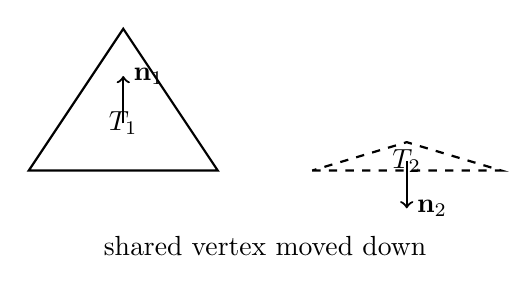
\begin{tikzpicture}[scale=1.2]
  % Original triangle
  \draw[thick] (0,0) -- (2,0) -- (1,1.5) -- cycle;
  \node at (1,0.5) {$T_1$};
  \draw[->,thick] (1,0.5) -- (1,1.0) node[right] {$\mathbf{n}_1$};

  % Flipped triangle after dedup
  \draw[thick,dashed] (3,0) -- (5,0) -- (4,0.3) -- cycle;
  \node at (4,0.1) {$T_2$};
  \draw[->,thick] (4,0.1) -- (4,-0.4) node[right] {$\mathbf{n}_2$};

  \node at (2.5,-0.8) {shared vertex moved down};
\end{tikzpicture}
\caption{Geometric flip: $T_1$ and $T_2$ share an edge with
consistent winding, but after dedup moves their shared vertex,
$T_2$'s normal flips while its winding stays consistent.}
\label{fig:flip}
\end{figure}

\texttt{fix\_winding}'s BFS pass propagates \emph{topological} winding
consistency (shared edges traversed in opposite directions), so it
cannot detect this geometric flip.  The signed-volume test also fails
for genus~$>0$ surfaces (e.g.\ torus), where the signed volume is
small and its sign does not reliably indicate global orientation.

\section{Solution}

\subsection{Relative Dedup Tolerance}

Replace the fixed \texttt{eps} with one scaled to the mesh's AABB
diagonal:
\[
  \texttt{eps} = \texttt{diag} \times 10^{-6}
\]
where
\[
  \texttt{diag} = \sqrt{(\max_x - \min_x)^2 + (\max_y - \min_y)^2 + (\max_z - \min_z)^2}.
\]

This adapts the merge tolerance to the mesh's actual size, preventing
over-merging at high resolutions.

\begin{lstlisting}
let diag = {
    let mut min = [f32::INFINITY; 3];
    let mut max = [f32::NEG_INFINITY; 3];
    for p in &positions {
        for i in 0..3 {
            min[i] = min[i].min(p[i]);
            max[i] = max[i].max(p[i]);
        }
    }
    let d = [max[0]-min[0], max[1]-min[1], max[2]-min[2]];
    (d[0]*d[0] + d[1]*d[1] + d[2]*d[2]).sqrt()
};
let eps = diag * 1e-6;
dedup_vertices(&mut positions, &mut indices, eps);
\end{lstlisting}

\subsection{Geometric Flip Detection}

After \texttt{fix\_winding} establishes topological consistency, a
second pass detects and corrects geometric flips:

\begin{enumerate}
  \item Compute per-face normals $\mathbf{n}_f$.
  \item Build vertex$\to$face adjacency.
  \item For each face $f$, compute the reference direction
        $\mathbf{r}_f = \sum_{f' \in \mathcal{N}(f)} \mathbf{n}_{f'}$,
        where $\mathcal{N}(f)$ is the set of faces sharing a vertex
        with $f$.
  \item If $\mathbf{n}_f \cdot \mathbf{r}_f < 0$, flip $f$'s winding.
\end{enumerate}

This correctly distinguishes:
\begin{itemize}
  \item \textbf{True geometric flips} (sphere: 1327/47234 faces) ---
        corrected.
  \item \textbf{Legitimate inward normals} (torus inner surface:
        22063/59310 faces) --- only 2039 are true flips, the rest
        are preserved because their neighbours also point inward.
\end{itemize}

\begin{lstlisting}
// Per-face normals
let mut face_normals: Vec<Vec3> = ...;
// Vertex -> face adjacency
let mut vert_faces: Vec<Vec<usize>> = ...;
// Detect flips
let mut to_flip = Vec::new();
for (fi, tri) in indices.chunks_exact(3).enumerate() {
    let n = face_normals[fi].normalize();
    let ref_sum: Vec3 = tri.iter()
        .flat_map(|&idx| vert_faces[idx as usize].iter())
        .filter(|&&nf| nf != fi)
        .map(|&nf| face_normals[nf])
        .sum();
    if ref_sum.length_squared() > 1e-12 && n.dot(ref_sum) < 0.0 {
        to_flip.push(fi);
    }
}
for &fi in &to_flip {
    indices.swap(fi*3+1, fi*3+2);
}
\end{lstlisting}

\section{Pipeline Summary}

The complete mesh construction pipeline in \texttt{from\_triangles}:

\begin{enumerate}
  \item \textbf{Dedup} --- merge duplicate vertices with
        $\texttt{eps} = \texttt{diag} \times 10^{-6}$; remove
        degenerate triangles.
  \item \textbf{Winding fix} --- BFS topological consistency +
        per-component signed volume.
  \item \textbf{Geometric flip fix} --- compare each face normal
        against neighbour normals; flip inconsistent faces.
  \item \textbf{Smooth normals} --- area-weighted normal averaging.
\end{enumerate}

\section{Results}

\begin{center}
\begin{tabular}{lrrrr}
\toprule
Mesh & depth & faces & geo-flips & status \\
\midrule
sphere       & 7 & 47234  & 1327 & OK \\
sphere       & 9 & 355818 & ---  & OK \\
torus        & 7 & 59310  & 2039 & OK \\
gyroid-sphere & 7 & 69836 & ---  & OK \\
\bottomrule
\end{tabular}
\end{center}

All meshes render correctly under back-face culling
(\texttt{cull\_mode = Back}, \texttt{front\_face = Ccw}) without
holes or dark triangles.

\end{document}
